
\section{Cost of Money}\label{sec:cost-of-money}

So far, we assumed that the cost of borrowing money is free.
However, in practice, loan platforms change interest.
For the flash loan of $b$ \asset, the adversary must pay an extra
$\betaasset b$ \asset in fees upon returning the borrowed \asset.
The adversary must also pay interest on the $z$ \stasset she borrowed.
The duration of the loan was $\Delta_z = t_5 - t_0$, so the
total loan amount to be repaid, including the principal and interest, is
$((1 + \rstasset)^{\Delta_z} + \betastasset) z$ \stasset.
Letting $f = ((1 + \rstasset)^{\Delta_z} + \betastasset)$ be the cost factor
of the loan, to recover this amount of \stasset and pay back the loan, the adversary must now
deposit $b' = \frac{b_0}{s_0}(1 - p\frac{b}{b_0 + b}) f z$ \asset
into the protocol.

Additionally, loans must also be overcollateralized.
Let $\gammastasset$ be the collateral ratio of a standard \stasset loan.
The adversary, using her whole initial capital $u$ as collateral can get a loan of
$z = \frac{u}{\gammastasset} \frac{s_0}{b_0}$ \stasset.
The loaned $z$ \stasset are then converted to $b^*=\frac{u}{\gammastasset}$ \asset.
To perform the attack, part of the $b^*$ \asset is used to exempt delegate $c$ like
before, but another part is now used to pay $\betaasset b$ for the flash loan cost.
Hence $c + \betaasset b \leq b^*$ and the adversary may now use up to
$b < \frac{u}{(\frac{1}{\phi} + \betaasset) \gammastasset}$ to move the price
of \stasset.


Taking into consideration the cost of borrowing money, the final profit of the attack is now
$\alpha = b^* - b' - qc - \betaasset b$ for the new values of $b^*$ and $b'$.
Solving for $\frac{d\alpha}{db} = 0$, like before, gives the optimal
$b = \sqrt{\frac{u f p b_0}{(\betaasset + \frac{q}{\phi})\gammastasset}} - b_0$,
which maximizes the adversary's profit, subject to the new constraints
$0 \leq b \leq \frac{u}{(\frac{1}{\phi} + \betaasset) \gammastasset}$.
Solving $\alpha \leq 0$ for $\frac{\phi}{q}$ and plugging in the adversarially optimal value for $b$
yields the new parametrization that keeps the protocol secure

\begin{gather*}
  \frac{\phi}{q} \leq \frac{b_0 \gammastasset}{f p u + f u - b_0 \betaasset \gammastasset - 2 u \sqrt{fp (f-1)} - u}\,.
\end{gather*}

 The cost of borrowing money increases when the collateral ratio
 $\gammastasset$, the flash loan cost factor $\betaasset$ or the loan cost factor $f$
 increase. While the cost of borrowing money goes up, the attack becomes less profitable
 for the adversary. Thus, the protocol can afford to increase $\frac{\phi}{q}$
 and still remain secure. This is illustrated in
 Figure~\ref{fig:plotf} for an adversary with $30\%$ market domination $\frac{u}{b0}$,
 and an adversary with $50\%$ market domination $\frac{u}{b0}$.
 While $f$ increases, the safe parameter $\frac{\phi}{q}$ can increase with it.
 The black line indicates where the attack becomes unprofitable for the adversary ($\alpha = 0$).
 The white area under the black line represents the configuration in which
 the protocol is secure in the rational model.

 \begin{figure}[htb]
   \centering
   \begin{subfigure}{0.49\textwidth}
     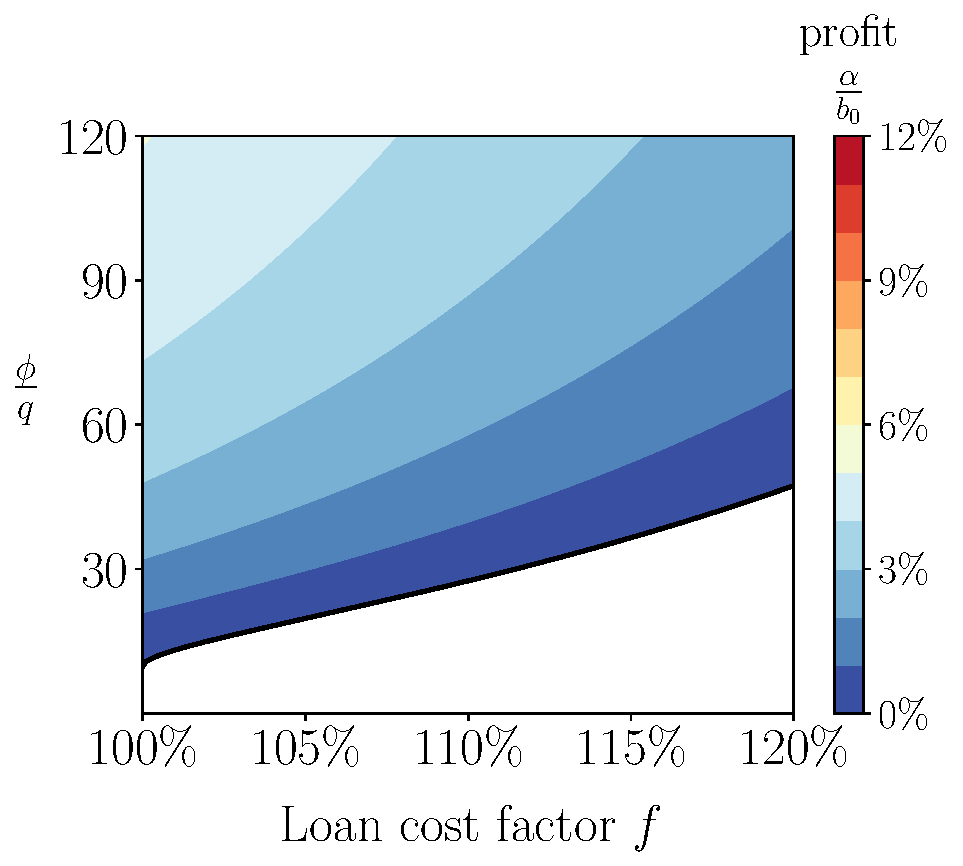
\includegraphics[width=\textwidth]{./figures/plotf30.pdf}
     \caption{Collateral $u$ is $30\%$ of $b_0$.}
     \label{fig:plotf30}
   \end{subfigure}
   \hfill
   \begin{subfigure}{0.49\textwidth}
     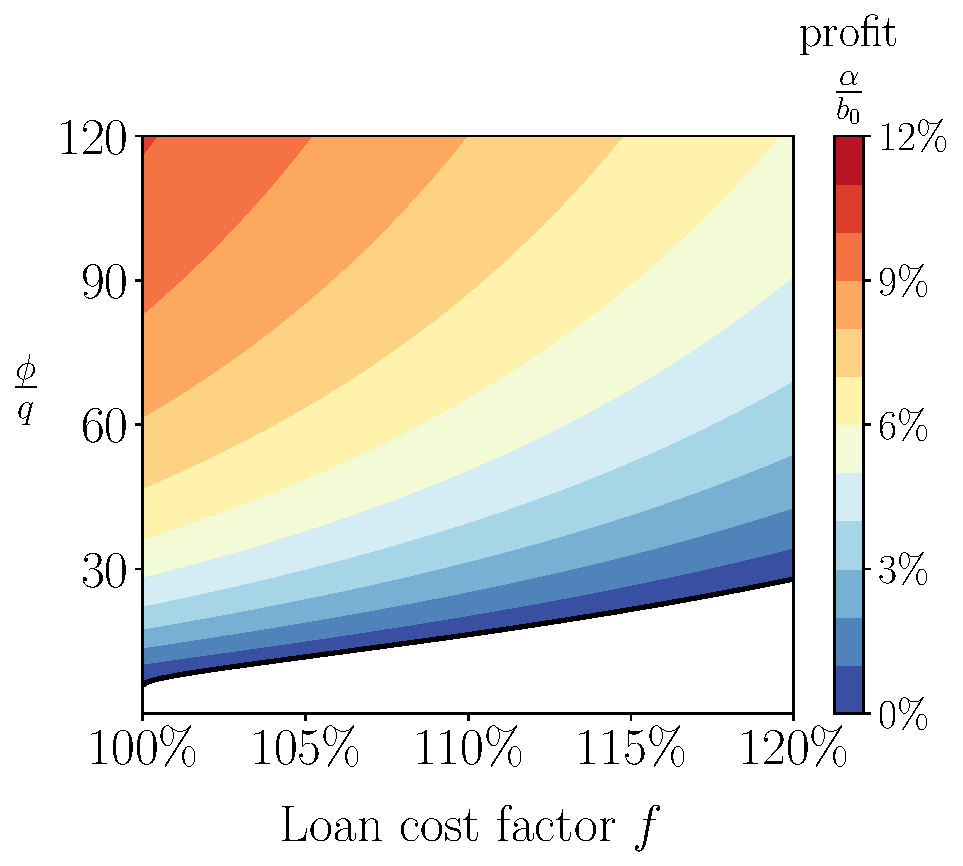
\includegraphics[width=\textwidth]{./figures/plotf50.pdf}
     \caption{Collateral $u$ is $50\%$ of $b_0$.}
     \label{fig:plotf50}
   \end{subfigure}
   \caption{Cost of borrowing and attack profitability.}
   \label{fig:plotf}
 \end{figure}

 As an illustration,
 we consider a blockchain with slashing percentage
 $p = 0.5$ and market conditions\footnote{Lido stETH borrowing rates
 on Aave~\cite{aave} as of 27 Jan, 2023.}
 with \asset flash loan cost factor $\betaasset = 0.0009$ and
 collateral ratio $\gammastasset = 146\%$.
 In Figure~\ref{fig:plotf} we plot the dependencies between $f$ and adversarial
 profit. At the time of writing, if the attack duration is $20$ sec, we have
 $f = 1 + 10^{-8}$.

We saw that, in practice, $f \simeq 1$, and money borrowing is almost free
for short durations. Free money borrowing makes the adversary more powerful
and her attack more profitable.
Hence, if a parameter $\frac{\phi}{q}$ keeps the protocol secure when money
borrowing is free ($f = 1$, $\betaasset = 0$, $\gammastasset = 1$),
the same parameter $\frac{\phi}{q}$ keeps the protocol secure even when
money borrowing is not free. This is illustrated in
Figure~\ref{fig:compare-f-plotu}. Safe values of parameter $\frac{\phi}{q}$
for $f = 1$, indicated by the black line, are also safe for $f > 1$
under any adversarial market domination $\frac{u}{b_0}$.

%TODO (tzinas): check if the same happens for β and γ
%TODO (camera ready?): add plots for γ and β

\begin{figure}[htb]
  \centering
  \hfill
  \begin{subfigure}{0.5\textwidth}
    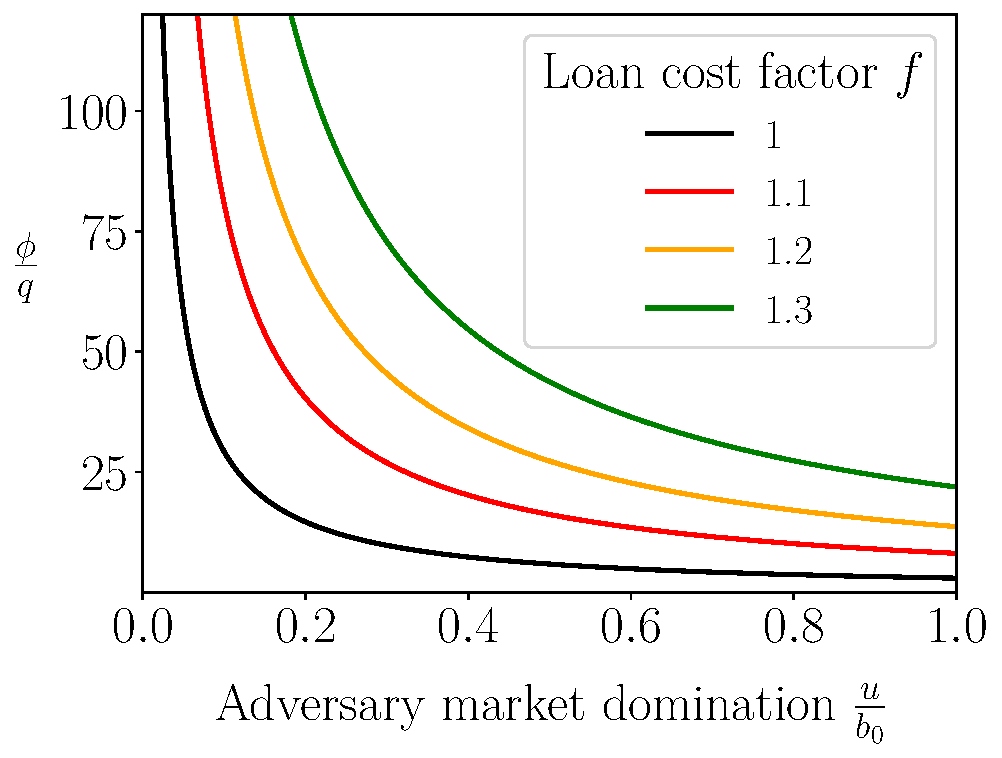
\includegraphics[width=\textwidth]{./figures/multiplef_plotu.pdf}
    \caption{Optimal $\frac{\phi}{q}$ system parametrizations
             for different adversarial market dominations $\frac{u}{b_0}$
             and market conditions $f$.}
    \label{fig:compare-f-plotu}
  \end{subfigure}
  \caption{Adversarial market domination and attack profitability.}
  \label{fig:plotu}
\end{figure}



\noindent
\textbf{Bookkeeping in USD.}
If the attacker wants to do bookkeeping in a more stable reference currency,
such as USD, the attack is still profitable. The attacker begins by buying
\asset for USD. At the end of the attack, the attacker sells \asset for USD.
Because the attack concerns a particular liquid staking protocol, and
not the whole \asset network, the price of \asset will likely not
be significantly affected by the attack at all.
This attack decreases the market confidence in \stasset,
but not in \asset.
In fact, because
the attack causes slashing of \asset, the supply of \asset is decreased
and the price of \asset with respect to the reference currency may
even increase.
Lastly, any price fluctuations of \asset with respect to USD will likely be
minor, as the attack has a short duration of a couple of seconds.

\noindent
\textbf{The Market price of \stasset.}\label{sec:stasset-price}
Let us consider the price $v$ of \stasset denominated in \asset in the market.
Because the option always exists to mint at a rate of $\frac{s_0}{b_0}$ by
depositing, the price of \stasset denominated in \asset in a perfectly
efficient market is $\frac{b_0}{s_0}$ at maximum. Otherwise, no
rational buyer would use the market. Hence, the market rate is
$v \leq \frac{b_0}{s_0}$.

There are two options to convert $s$ \stasset to \asset: either sell
at the market rate to obtain $b = v s$ \asset, or use the redemption mechanism.
Using the redemption mechanism, the \assets become available after
time $\delta$.
Initially, using $s$ \stasset, a redemption is made of $b' = s \frac{b_0}{s_0}$
delegated assets. To get $b$ \asset immediately (and avoid having to wait
for the unbonding period), a loan of $b$ \asset is taken~\cite[p.~13]{liquid-staking-report} and
repayed after duration $\delta$.
The amount of \asset that needs to be paid back,
including principal and interest, is $((1 + \rasset)^\delta + \betaasset)b$ \asset.
We set this amount to be equal to $b'$, the amount of \assets that will be
unbonded after $\delta$ time. Solving for $b$, we get
$b = s \frac{b_0}{s_0 ((1 + \rasset)^\delta + \betaasset)}$.
Therefore, in an efficient market $v \geq \frac{b_0}{s_0 ((1 + \rasset)^\delta + \betaasset)}$.
We deduce that the bounds for an efficient market of \asset and \stasset are

\[
  \frac{b_0}{s_0 ((1 + \rasset)^\delta + \betaasset)} \leq v \leq \frac{b_0}{s_0}\,.
\]

The longer the duration $\delta$, the larger the potential price deviation
(c.f. the empirical analysis in
\emph{Liquid Staking: Basis Determinants and Price Discovery}~\cite{scharnowski2022liquid}).
Such loans are available in practice and some
protocols~\cite[\S5]{parallel}\cite{marinade-matching} even automate this process.

It is also possible to use the principle of \emph{remittances}
(matching)~\cite[\S5]{parallel}\cite{marinade-matching} to match depositing and
redeeming parties, so that the redeeming party does not have to incur any unbonding delay.
If the redeemed amounts exceed the deposited amounts, some amounts will necessarily incur
a delay. However, the above bounds may effectively be tighter than $\delta$ due to
a shorter effective unbonding duration.
